% !TEX root = ../math407-notes.tex
% Transcribed from handwritten notes (1.1 Generalities, 1.2 Equations Over a
% Finite Field, 1.3 Quadratic Reciprocity).

\section{Preliminaries}

Let $K$ be a field. Then, $(K^\times, \cdot)$ is an abelian group. We have a homomorphism $\Z \to K$ by $1 \mapsto 1$, and its image $\Img(\Z) \subset K$ is a domain. So, either
$$\Z \hookrightarrow K \quad (\Char K = 0), \quad \text{or} \quad \Z \twoheadrightarrow \Z/p\Z \hookrightarrow K \quad (\Char K = p).$$
In the first case, $\Z \hookrightarrow K$ is equivalent to $\Q \hookrightarrow K$.

\begin{notebox*}[Observation]
    If $K$ has characteristic $p$, then there exists a ring homomorphism $\phi : K \to K$ given by $\phi(x) = x^p$, since
    $$\phi(x+y) = (x+y)^p = x^p + y^p + 0.$$
    Since $K$ is a field, $\phi$ must be injective, since the kernel must be trivial.
\end{notebox*}

\begin{defn}
    Let $K$ have characteristic $p$. Then, $K$ is \textbf{perfect} if $\phi : K \to K$ is an automorphism.
\end{defn}

\begin{ex}
    \begin{enumerate}
        \item An algebraically closed field $K = \bar K$ of characteristic $p$.
        \item $\F_p = \Z/p\Z$.
    \end{enumerate}
\end{ex}

\begin{defn}
    The map $\phi$ is called the \textbf{Frobenius map}.
\end{defn}

\begin{thm}
    Let $R$ be a finite domain. Then, $R$ must be a field.
\end{thm}

\begin{proof}
    For $x \neq 0$, the map $\phi_x : R \to R$ given by $y \mapsto xy$ is a bijection, so $\phi_x(y) = 1$ has a solution.
\end{proof}

\begin{thm}
    Let $K$ be a finite field.
    \begin{enumerate}[(1)]
        \item $\Char K = p > 0$, and $|K| = p^f$.
        \item Let $q = p^f$, $f \geq 1$, and let $\Omega$ be an algebraically closed field of characteristic $p$. Then, there exists a unique subfield of $\Omega$ of order $q$, denoted
        $$\F_q = \{\text{roots of } x^q - x \text{ in } \Omega\}.$$
        \item Any finite field of order $q$ is isomorphic to $\F_q$.
    \end{enumerate}
\end{thm}

\begin{proof}
    \hfill
    \begin{enumerate}[(1)]
        \item $K$ has characteristic $p$ because $\Q \not\hookrightarrow K$, hence $\Z/p\Z \hookrightarrow K$. So, $K$ is a vector space over $\Z/p\Z$, and $\dim(K)$ over $\F_p$ is finite. The degree of the extension is the same as the dimension of the vector space, so $|K| = p^f$, where $f$ is the degree.
        \item Let $\Omega$ be an algebraically closed field of characteristic $p$, and let $\phi : \Omega \to \Omega$ be given by $\phi(x) = x^q$. Then, $\phi$ is injective, and surjective by algebraic closure, hence is an automorphism. For any automorphism $T : E \to E$ of a field, the set
        $$F = \{x \in E \mid T(x) = x\} \subset E$$
        is a subfield. Let $\F_q$ be the set of elements fixed by $\phi$. All of its elements are roots of $x^q - x$, which has at most $q$ roots. Note that
        $$\frac{d}{dx}(x^q - x) = qx^{q-1} - 1 = -1 \neq 0,$$
        hence $x^q - x$ has no repeated roots. That is, $|\F_q| = q$.
    \end{enumerate}
\end{proof}

\begin{lem}
    $\F_{p^e} \subset \F_{p^f} \iff e \mid f$.
\end{lem}

\begin{proof}
    This follows by degree considerations.
\end{proof}

\begin{proof}[Proof of (3)]
    Given $K$ with $|K| = q$, there exists an algebraically closed field $\Omega$ containing $K$. For example, we could take $\Omega = \bar K$. Then, $\Omega$ has characteristic $p$. Let
    $$\F_q = \{a \in \Omega : a^q = a\} \subset \Omega.$$
    We want to show that $K = \F_q$. We have $a^q - a = a(a^{q-1} - 1)$. Let $a \in K \setminus \{0\}$. Then, $a \in K^\times$ and $|K^\times| = q - 1$, hence $a^{q-1} = 1$, so $a \in \F_q$. Also, $0 \in \F_q$, so $K \subseteq \F_q$. However, $|K| = |\F_q|$, hence $K = \F_q$.
\end{proof}

\begin{ex}
    \begin{enumerate}
        \item $\F_{3^2} \cong \F_3[x]/(x^2+1)$.
        \item More generally, $\F_p[x]/(x^2+1) = \F_{p^2} \iff p \equiv 3 \pmod 4$.
        \item $\F_{3^3} \cong \F_3[x]/(x^3+2x+1)$.
    \end{enumerate}
\end{ex}

\begin{notebox*}[Recall]
    $(\Z,+)$ has no non-zero elements of finite order.
\end{notebox*}

\begin{defn}
    For $G$ abelian, let $G_t = \{g \in G : |g| < \infty\}$, called the \textbf{torsion} of $G$.
\end{defn}

\begin{ex}
    $\Q/\Z$ is a torsion group.
\end{ex}

\begin{defn}
    Let $A$ be an abelian group. $A$ is \textbf{divisible} if for every map $A \to A$ given by $a \mapsto na$ with $n \in \Z \setminus \{0\}$ (where $na = a + \overset{n}{\cdots} + a$), the map is surjective. Note that these maps are always homomorphisms.
\end{defn}

\begin{ex}
    \begin{enumerate}
        \item $(\Z,+)$ is not divisible.
        \item $(\Q,+)$ is divisible.
        \item $\Q/\Z$ is divisible.
    \end{enumerate}
\end{ex}

\begin{defn}
    $A$ is \textbf{uniquely divisible} if all of those maps are automorphisms.
\end{defn}

\begin{ex}
    Consider the torsion of $(K^\times, \times)$ for the following fields $K$:
    \begin{center}
        \begin{tabular}{c|c}
            $K$ & Torsion of $K^\times$ \\ \hline
            $\Q$ & $\{\pm 1\}$ \\
            $\R$ & $\{\pm 1\}$ \\
            $\C$ & $\{\text{roots of unity}\} \cong \Q/\Z$ \\
            $\bar \Q$ & $\Q/\Z$
        \end{tabular}
    \end{center}
\end{ex}

\begin{thm}
    $(\F_q)^\times$ is cyclic. For $q = p$, this is equivalent to there being a primitive root modulo $p$.
\end{thm}

\begin{proof}
    \begin{notebox*}[Fact]
        Let $C_n = \angles{\sigma}$ be the cyclic group of order $n$, so $|\sigma| = n$. Then, $|\sigma^k| = \frac{n}{(k,n)}$. So,
        $$\#\{x \in C_n : |x| = n\} = \varphi(n).$$
        That is, $C_n$ has exactly $\varphi(n)$ generators.
    \end{notebox*}

    \begin{lem}
        Let $n \in \N$. Then, $n = \sum_{d \mid n} \varphi(d)$.
    \end{lem}

    \begin{proof}
        Let $\Phi_d = \{\text{elements of order } d \text{ in } C_n\}$. Then,
        $$C_n = \bigsqcup_{d \mid n} \Phi_d \implies \# C_n = \sum_{d \mid n} \# \Phi_d = \sum_{d \mid n} \varphi(d).$$
    \end{proof}

    \begin{lem}[Recognition of Finite Cyclic Groups]
        Let $H$ be finite and abelian, with $\# H = n$. Suppose that for all $d \mid n$, we have $\#\{a \in H : a^d = 1\} \leq d$. Then, $H \cong C_n$.
    \end{lem}

    \begin{proof}
        Let $d \mid n$, and let $H_d = \{a \in H : a^d = 1\}$. If there exists $x \in H$ of order $d$, then $\angles{x}$ has size $d$, and all elements $y \in \angles{x}$ satisfy $y^d = 1$. So, any $z \in H$ with $z^d = 1$ must be in $\angles{x}$. That is, $H_d \leq \angles{x}$. Hence, all elements of order $d$ are generators of $\angles{x} \leq H$, so there are exactly $\varphi(d)$ elements of order $d$ in $H$. So, if $d \mid n$, the number of elements of order $d$ in $H$ is either $0$ or $\varphi(d)$. Since $\# H = \sum_{d \mid n} \varphi(d)$, by counting we need an element of every order. In particular, $H$ has an element of order $n$.
    \end{proof}

    Now, let $H = (\F_q)^\times$, $n = q - 1$, and $H_d = \{a \in \F_q^\times : a^d = 1\}$. That is, $H_d = \{\text{roots of } x^d - 1 = 0\}$, and $x^d - 1$ has at most $d$ roots. So, $\# H_d \leq d$, hence $H$ is cyclic.
\end{proof}

\begin{notebox*}
    With the same argument, for any field $K$, any finite subgroup $H \leq K^\times$ is cyclic.
\end{notebox*}

\begin{ex}
    In $\F_5[x]$, we have $x^2 + 1 = (x+2)(x-2)$, so $\F_5[x]/(x^2+1) = \F_5[x]/(x+2)(x-2)$. Note that we have
    \[\begin{tikzcd}
        {\F_5[x]} && {\F_5[x]/(x+2)} \\
        \\
        {\F_5[x]/(x^2+1)}
        \arrow[two heads, from=1-1, to=1-3]
        \arrow[two heads, from=1-1, to=3-1]
        \arrow["{\exists}"', dashed, from=3-1, to=1-3]
    \end{tikzcd}\]
    where the dashed map exists because $x^2 + 1 \mapsto 0$. So, we get maps
    $$\F_5[x]/(x^2+1) \to \F_5[x]/(x+2) \cong \F_5, \qquad \F_5[x]/(x^2+1) \to \F_5[x]/(x-2) \cong \F_5,$$
    which combine to give $\F_5[x]/(x^2+1) \to \F_5 \times \F_5$.
\end{ex}

\section{Equations Over a Finite Field}

We look at equations over finite fields, and search for solutions.

\begin{defn}
    Let $g(x_1,\dots,x_n) \in \Z[x_1,\dots,x_n]$. The \textbf{solution set} of $g$ is
    $$V(g) = \{(a_1,\dots,a_n) \in \Z^n \mid g(a_1,\dots,a_n) = 0\}.$$
\end{defn}

\begin{ex}
    Let $f(x) = x^2 + 1$. If $f(a) = 0$, then $f(a) \equiv 0 \pmod p$ for all $p$. That is, $f$ has a root in $\F_p$. Let
    $$V_p(f) = \{\bar a \in \F_p : f(\bar a) = 0\}.$$
    If we can show $V_p(f)$ is empty for some prime $p$, then $V(f)$ is empty. Indeed, $V_3(f) = \emptyset$, hence $V(f) = \emptyset$.
\end{ex}

\begin{ex}
    Let $V(h) = \{(a,b,c) \mid a^5 + b^5 + c^5 = 0\}$. Does $V_p(h)$ non-empty imply $V(h)$ non-empty? \textbf{No.}
\end{ex}

\begin{notebox*}[Questions]
    \begin{enumerate}[(1)]
        \item Is every element of $\F_q$ a sum of $2$ squares? That is, does $x^2 + y^2 - a$ have a root for all $a \in \F_q$?
        \item Let $g(x,y,z) = 3x^2 + 5y^2 + 7z^2$, and let $a_p = |V_p(g)|$ be the number of solutions of $g$ in $\F_p$. What can we say about $a_p$? Is $\lim_{p \to \infty} a_p = \infty$, or is it bounded?
    \end{enumerate}
\end{notebox*}

\subsection{The Chevalley-Warning Theorem}

\begin{thm}[Chevalley-Warning Theorem][label=thm:chevalley-warning]
    Let $K = \F_q$ be a finite field, $R = K[x_1,\dots,x_n]$, and $f_1,\dots,f_r \in R$. Let $d = \deg f_1 + \cdots + \deg f_r$, and
    $$V = \{(a_1,\dots,a_n) \in K^n : f_j(a_1,\dots,a_n) = 0 \text{ for all } 1 \leq j \leq r\}.$$
    If $d < n$, then $\# V \equiv 0 \pmod p$.
\end{thm}

\begin{cor}
    Suppose in addition that $f_1,\dots,f_r$ have no constant term. Then, $V$ is non-empty because of the zero solution, hence $\# V \geq p$.
\end{cor}

\begin{cor}
    Let $f(x,y,z) = ax^2 + by^2 + cz^2 + dxy + exz + gyz$ be a quadratic form. Observe that $f(\lambda x, \lambda y, \lambda z) = \lambda^2 f(x,y,z)$. Since $f(0,0,0) = 0$, $f$ has a non-trivial solution in $\F_q$ as well.
\end{cor}

We can use this to answer question (1). Fix $a \in \F_q$, and consider $g(x,y,z) = x^2 + y^2 - az^2$. The theorem also answers question (2).

We can prove Chevalley-Warning with power sums.

\begin{ex}
    Let $K = \F_{11} = \{0,\dots,10\}$. For $m \geq 0$, let $f(x) = x^m$, and let $S_m = \sum_{a \in \F_{11}} a^m$. Note that
    $$S_0 = 0 \ (\text{taking } 0^0 = 1), \qquad S_1 = 0, \qquad S_{10} = 0 + 1 + \cdots + 1 = -1.$$
    What are $S_2$ and $S_3$?
\end{ex}

\begin{notebox*}[Observe]
    For a group $G$ and $g_0 \in G$, the map $g \mapsto g_0 g$ is a bijection.
\end{notebox*}

\begin{lem}[][label=lem:power-sums]
    Let $K = \F_q$ have characteristic $p$, with $q = p^f$. Let $S_m = \sum_{a \in K} a^m$, and more generally, if $f(x) = x^m$, let $S(f) = \sum_{a \in K} f(a)$. Then,
    \begin{enumerate}[(1)]
        \item $S_0 = 0$.
        \item If $m \geq 1$ and $q - 1 \mid m$, then $S_m = -1$.
        \item If $m \geq 1$ and $q - 1 \nmid m$, then $S_m = 0$.
    \end{enumerate}
\end{lem}

\begin{proof}
    \hfill
    \begin{enumerate}[(1)]
        \item $m = 0$ is clear.
        \item Suppose $q - 1 \mid m$. Then, for $a \in \F_q$, $a = 0 \implies a^m = 0$. Also, $a \neq 0 \implies a^m = 1$, since $\# \F_q^\times = q - 1$. So, $S_m = 0 + 1 + 1 + \cdots + 1 = -1$.
        \item Suppose $q - 1 \nmid m$. Then, there exists $y \neq 0$ in $K$ such that $y^m \neq 1$, because $K^\times$ is cyclic. Now, consider the map $K^\times \to K^\times$ given by $a \mapsto ay$, which is a bijection. Then,
        $$S_m = \sum_{a \in K^\times} a^m = \sum_{a \in K^\times} (ay)^m = y^m \sum_{a \in K^\times} a^m = y^m S_m.$$
        Thus, $(1 - y^m) S_m = 0$, and $1 - y^m \neq 0$, hence $S_m = 0$.
    \end{enumerate}
\end{proof}

\begin{lem}[][label=lem:monomial-sum]
    Let $g(x_1,\dots,x_n) \in R$ be a monomial, i.e. $g = x_1^{e_1} \cdots x_n^{e_n}$, and suppose $\sum e_i < (q-1)n$. As $g$ is a function $K^n \to K$, we can consider
    $$S(g) = \sum_{(a_1,\dots,a_n) \in K^n} g(a_1,\dots,a_n).$$
    Then, $S(g) = 0 \in K$.
\end{lem}

\begin{proof}
    By assumption, there exists $i$ with $e_i < q - 1$. Without loss of generality, suppose $i = 1$. Then,
    $$S(g) = \sum a_1^{e_1} \cdots a_n^{e_n} = \sum_{a_2,\dots,a_n} a_2^{e_2} \cdots a_n^{e_n} \paren{\sum_{a_1 \in K} a_1^{e_1}},$$
    but that last factor is $0$ by \Cref{lem:power-sums}, because $e_1 = 0$ or $q - 1 \nmid e_1$.
\end{proof}

\begin{ex}
    Let $W \subset \R$. The \textbf{characteristic function} of $W$ is
    $$\chi_W(x) = \case{1 & x \in W \\ 0 & x \notin W}$$
\end{ex}

\begin{defn}
    Let
    $$P(x_1,\dots,x_n) = \prod_{i=1}^r \paren{1 - f_i^{q-1}},$$
    where $f_1,\dots,f_r$ are the polynomials in \Cref{thm:chevalley-warning}. Note that $\deg f_i^{q-1} = (q-1)\deg f_i$, so $\deg P = (q-1)d < (q-1)n$.
\end{defn}

Observe that
$$(a_1,\dots,a_n) \in V \implies P(a_1,\dots,a_n) = 1, \qquad (a_1,\dots,a_n) \notin V \implies P(a_1,\dots,a_n) = 0.$$
Hence, $P$ is a \textbf{characteristic function} of $V$.

\begin{lem}
    $S(P) \equiv \# V \pmod p$. (Not $=$, because we are working mod $p$.)
\end{lem}

\begin{proof}[Proof of \Cref{thm:chevalley-warning}]
    To finish the proof, we want to show that $S(P) \equiv 0$. Write
    $$P(x_1,\dots,x_n) = \sum c_{e_1,\dots,e_n} x_1^{e_1} \cdots x_n^{e_n}.$$
    If $g$ is one such monomial, then $\deg g < (q-1)n$, hence $S(g) = 0$ by \Cref{lem:monomial-sum}. Therefore, $S(P) = \sum S(g) = 0$.
\end{proof}

\begin{ex}
    Let $K = \F_5$, $f = x + y - 1$, and $V = V(f)$. The points of $V$ are circled below.
    \begin{center}
        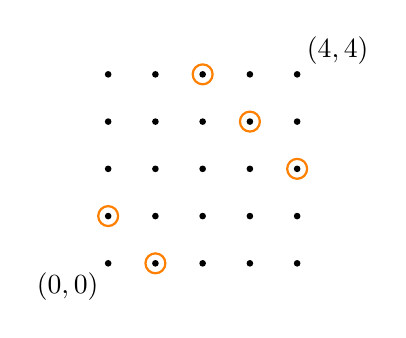
\begin{tikzpicture}[scale=0.6]
            \foreach \x in {0,...,4} \foreach \y in {0,...,4} \fill (\x,\y) circle (2pt);
            \foreach \p in {(1,0),(0,1),(4,2),(3,3),(2,4)} \draw[thick, color=orange] \p circle (6pt);
            \node[below left] at (0,0) {$(0,0)$};
            \node[above right] at (4,4) {$(4,4)$};
        \end{tikzpicture}
    \end{center}
\end{ex}

\begin{thm}[Warning's Theorem]
    Let $K = \F_q = \F_{p^f}$, $f_1,\dots,f_r \in K[x_1,\dots,x_n]$, $d = \sum \deg f_i$, and $V = V(f_1) \cap \cdots \cap V(f_r)$. If $V \neq \emptyset$, then $\# V \geq q^{n-d}$.
\end{thm}

\section{Quadratic Reciprocity}

\subsection{Preliminaries}

We want to understand the perfect squares in $\F_q^\times$.

\begin{thm}[][label=thm:squares-index-two]
    Let $q = p^f$.
    \begin{enumerate}[(1)]
        \item If $p = 2$, all elements of $\F_q$ are squares.
        \item If $p > 2$, then the squares form a subgroup of $\F_q^\times$ of index $2$.
    \end{enumerate}
\end{thm}

\begin{proof}[Proof of (1)]
    Let $K$ have characteristic $2$. Then, the map $K \to K$ given by $x \mapsto x^2$ is a homomorphism of fields. So, it must be injective, and if $K$ is finite, then the map is surjective.
\end{proof}

\begin{proof}[Proof of (2)]
    Let $\psi : \F_q^\times \to \{\pm 1\}$ be given by $\psi(a) = a^{\frac{q-1}{2}}$. Then, $\psi$ is a homomorphism of groups. Let $c = \psi(a) = a^{\frac{q-1}{2}}$. Then, $c^2 = 1$, hence $c$ is a root of $x^2 - 1 = 0$. So, $a^{\frac{q-1}{2}}$ can only be $\pm 1$.

    Now, we claim $\ker \psi = \{a \in \F_q^\times \mid \psi(a) = 1\}$ is the set of squares in $\F_q^\times$. Suppose $a \in (\F_q^\times)^2$, i.e. $a = b^2$ for some $b \in \F_q^\times$. Then, $\psi(a) = 1$. Hence, $(\F_q^\times)^2 \leq \ker \psi$. Conversely, if $a \in \ker \psi$, we need to show $a \in (\F_q^\times)^2$.

    Is $\psi$ onto? Yes: $\F_q^\times$ is cyclic, so it has a generator $g$, hence $g^{\frac{q-1}{2}} = -1$. Hence, $\F_q^\times / \ker \psi \cong \{\pm 1\}$, so $|\ker \psi| = \frac{q-1}{2}$. This means $\angles{g^2} = \ker \psi$ (a cyclic group has only one subgroup of a given order), so everything in $\ker \psi$ is a square.
\end{proof}

\begin{defn}
    Let $A, B, C$ be abelian groups, and consider homomorphisms
    $$0 \to A \arr[f] B \arr[g] C \to 0$$
    with $g(f(a)) = 0$ for all $a \in A$. This is a \textbf{sequence}. We say it's \textbf{exact on the left} if $f$ is injective, and \textbf{exact on the right} if $g$ is surjective. We say it's \textbf{exact in the middle} if $\Img f = \ker g$. We say it's an \textbf{exact sequence} if all $3$ hold.
\end{defn}

\begin{prop}
    If we have an exact sequence as above, then $B/\ker g \cong C$, so $B/\Img f \cong C$. Since $A \cong \Img f$, we have $B/A \cong C$.
\end{prop}

\begin{ex}
    The following sequences are exact:
    \begin{enumerate}
        \item $0 \to \Z \arr[\cdot 2] \Z \arr[\text{mod } 2] \Z/2\Z \to 0$
        \item $0 \to \Z \to \Q \to \Q/\Z \to 0$
        \item $1 \to \{\pm 1, \pm i\} \arr[\times] \C^\times \arr[a^4] \C^\times \to 1$. (We use $1$ instead of $0$ as a convention, since $1$ is the identity.)
        \item $1 \to (\F_q^\times)^2 \to \F_q^\times \arr[\psi] \{\pm 1\} \to 1$, where $\psi$ is the map from before.
    \end{enumerate}
\end{ex}

\begin{ex}
    Let $G$ be abelian, and consider the map $\phi_n : G \to G$ given by $\phi_n(a) = a^n$. Then, $\ker \phi_n = \{g \in G : g^n = e\}$. For example, we have the exact sequence
    $$1 \to \{\pm 1\} \to \F_q^\times \arr[\phi_2] (\F_q^\times)^2 \to 1.$$
\end{ex}

\begin{notebox*}[Principle]
    To check if $a \in \F_q^\times$ is a square, we need to check whether $\sqrt{a} = b \in \Omega$ satisfies $b^{q-1} = 1$.
\end{notebox*}

\subsection{The Legendre Symbol}

We now only consider prime fields.

\begin{defn}
    Let $a \in \Z$, and $p$ be prime. The \textbf{Legendre symbol} is
    $$\leg{a}{p} = \case{1 & \text{if } a \text{ is a square in } \F_p \\ -1 & \text{otherwise}}$$
    for $p \nmid a$, and $\leg{0}{p} = 0$.
\end{defn}

\begin{notebox*}
    $\leg{a}{p}$ depends only on the congruence class of $a$ modulo $p$.
\end{notebox*}

\begin{prop}
    If $b \in \Omega$ satisfies $b^2 = a \in \F_p^\times$, then
    $$\psi(a) = a^{\frac{p-1}{2}} = b^{p-1},$$
    which is $1$ if and only if $b \in \F_p$. So, $\leg{a}{p} = b^{p-1} \in \F_p^\times$, i.e. $\psi(a) = \leg{a}{p}$. Since $\psi(ab) = \psi(a)\psi(b)$, we have
    $$\leg{ab}{p} = \leg{a}{p} \leg{b}{p}.$$
\end{prop}

\begin{prop}
    We have
    $$\leg{a}{p} = \case{0 & a = 0 \\ 1 & a \text{ is a square} \\ -1 & a \text{ is not a square}}$$
    so $\sum_{a \in \F_p} \leg{a}{p} = 0$.
\end{prop}

Now, it helps to compute the Legendre symbol in special cases. In particular, we want to compute $\leg{-1}{p}$ and $\leg{2}{p}$.

\begin{defn}
    Let $n \in \Z$ be odd. We define two maps:
    $$\veps(n) \in \Z/2\Z, \quad \veps(n) = \frac{n-1}{2} \bmod 2 = \case{0 & n \equiv 1 \pmod 4 \\ 1 & n \equiv 3 \pmod 4}$$
    $$\omega(n) \in \Z/2\Z, \quad \omega(n) = \frac{n^2-1}{8} \bmod 2 = \case{0 & n \equiv \pm 1 \pmod 8 \\ 1 & n \equiv \pm 3 \pmod 8}$$
\end{defn}

\begin{thm}[][label=thm:legendre-special]
    Let $p$ be an odd prime. Then,
    \begin{enumerate}[(1)]
        \item $\leg{-1}{p} = (-1)^{\veps(p)}$, so $\leg{-1}{p} = 1 \iff p \equiv 1 \pmod 4$.
        \item $\leg{2}{p} = (-1)^{\omega(p)}$, so $\leg{2}{p} = 1 \iff p \equiv \pm 1 \pmod 8$.
    \end{enumerate}
\end{thm}

\begin{proof}
    \hfill
    \begin{enumerate}[(1)]
        \item If $-1 = c^2$ in $\F_p^\times$, then $c$ has order $4$. This requires $4 \mid p - 1$, i.e. $p \equiv 1 \pmod 4$, and further $p \equiv 3 \pmod 4 \implies \leg{-1}{p} = -1$. Now, suppose $p \equiv 1 \pmod 4$. Since $\F_p^\times$ is cyclic, let $\F_p^\times = \angles{g}$, so $g^{\frac{p-1}{4}} = g^k$ has order $4$. So, $-1 = (g^k)^2$, hence $\leg{-1}{p} = 1$.
        \item Let $\alpha \in \Omega$ be a primitive $8\th$ root of unity. So, $\alpha^8 = 1$, and
        \begin{enumerate}[(i)]
            \item $\alpha^4 = -1$.
            \item $\alpha^2 + \alpha^{-2} = 0$. Indeed, $(\alpha^2 + \alpha^{-2})^2 = \alpha^4 + \alpha^{-4} + 2\alpha^2\alpha^{-2} = -1 + (-1) + 2 = 0$.
            \item Let $y = \alpha + \alpha^{-1}$. Then, $y^2 = 2$. Indeed, $y^2 = (\alpha + \alpha^{-1})^2 = \alpha^2 + \alpha^{-2} + 2\alpha\alpha^{-1} = 0 + 2 = 2$.
        \end{enumerate}
        To compute $\leg{2}{p}$, we need $2^{\frac{p-1}{2}} = y^{p-1}$. Now,
        $$y^p = (\alpha + \alpha^{-1})^p = \alpha^p + \alpha^{-p}.$$
        If $p = 8k + 1$, then $y^p = \alpha^{8k+1} + \alpha^{-1-8k} = \alpha + \alpha^{-1} = y$, so $y^{p-1} = 1$, hence $y \in \F_p^\times$. Hence, $\leg{2}{p} = 1$. The case $p = 8k - 1$ is similar.

        If $p = 8k + 5$, then
        $$y^p = \alpha^{8k+5} + \alpha^{-5-8k} = \alpha^5 + \alpha^{-5} = \alpha\alpha^4 + \alpha^{-1}\alpha^{-4} = -(\alpha + \alpha^{-1}) = -y,$$
        hence $y^p = -y$, so $y^{p-1} = -1$, showing $\psi(2) = -1$, and thus $\leg{2}{p} = -1$. The case $p = 8k - 5$ is similar.
    \end{enumerate}
\end{proof}

\begin{ex}
    Let $f(x) = ax^2 + bx + c \in \F_p[x]$, with $p \nmid a$. By the quadratic formula, $f$ has roots $\iff \leg{b^2 - 4ac}{p} = 1$. In particular, $\F_p[x]/(f)$ is a field $\iff \leg{b^2-4ac}{p} = -1$.
\end{ex}

\subsection{Quadratic Reciprocity}

\begin{thm}[Quadratic Reciprocity (Carl ``G-money'' Gauss)][label=thm:qr]
    Let $p, \ell$ be odd primes, $p \neq \ell$. Then,
    $$\leg{p}{\ell} \leg{\ell}{p} = (-1)^{\veps(p)\veps(\ell)} = (-1)^{\frac{p-1}{2} \cdot \frac{\ell-1}{2}}.$$
\end{thm}

\begin{cor}
    $\leg{p}{\ell} = \leg{\ell}{p}$, unless $p \equiv \ell \equiv 3 \pmod 4$.
\end{cor}

\begin{ex}
    Let $\ell = 4003$ and $p = 5$. Computing $\leg{5}{4003}$ directly is hard, but $\leg{4003}{5}$ is easy:
    $$-1 = \leg{4003}{5} = \leg{5}{4003}.$$
\end{ex}

\begin{proof}[Proof of \Cref{thm:qr}]
    Fix $\F_p$, with $\F_p \subset \Omega$ algebraically closed. Let $\omega$ be a primitive $\ell\th$ root of unity in $\Omega$.

    \begin{lem}[][label=lem:qr0]
        $1 + \omega + \omega^2 + \cdots + \omega^{\ell - 1} = 0$.
    \end{lem}

    Also, recall that $\leg{a}{p} = b^{p-1}$ if $b^2 = a$.

    Consider the (well-defined) function $\F_\ell \to \{\pm 1\}$ given by $a \mapsto \leg{a}{\ell}$. Note that $\omega^a$ depends only on $a \bmod \ell$, so we can also consider the function $\F_\ell \to \Omega$ given by $a \mapsto \omega^a$. Let
    $$y = \sum_{a \in \F_\ell} \leg{a}{\ell} \omega^a \in \Omega.$$
    This $y$ is called a \textbf{Gauss sum}.

    \begin{lem}[][label=lem:qr1]
        $y^2 = (-1)^{\veps(\ell)} \ell$.
    \end{lem}

    \begin{lem}[][label=lem:qr2]
        $y^{p-1} = \leg{p}{\ell}$.
    \end{lem}

    We will show these lemmas imply quadratic reciprocity, and then prove them. As $y^2 = (-1)^{\veps(\ell)}\ell$, we get from the note above (with $b = y$) and \Cref{lem:qr2} that
    $$\leg{(-1)^{\veps(\ell)}\ell}{p} = y^{p-1} = \leg{p}{\ell}.$$
    As the Legendre symbol is multiplicative,
    $$\leg{(-1)^{\veps(\ell)}\ell}{p} = \leg{-1}{p}^{\veps(\ell)} \leg{\ell}{p} = \paren{(-1)^{\veps(p)}}^{\veps(\ell)} \leg{\ell}{p}.$$
    So, $\leg{p}{\ell} = (-1)^{\veps(p)\veps(\ell)} \leg{\ell}{p}$, hence
    $$\leg{p}{\ell}\leg{\ell}{p} = (-1)^{\veps(p)\veps(\ell)},$$
    as desired.
\end{proof}

\begin{proof}[Proof of \Cref{lem:qr0}]
    As $\omega$ is a primitive $\ell\th$ root of $1$, $\omega$ is a root of
    $$\frac{x^\ell - 1}{x - 1} = 1 + x + \cdots + x^{\ell - 1},$$
    so $1 + \omega + \cdots + \omega^{\ell - 1} = 0$.
\end{proof}

\textit{(Rama really wants us to understand this proof.)}

\begin{proof}[Proof of \Cref{lem:qr2}]
    Let $y = \sum_{a \in \F_\ell} \leg{a}{\ell} \omega^a$. As $\Omega$ has characteristic $p$,
    $$y^p = \paren{\sum \leg{a}{\ell} \omega^a}^p = \sum_{a \in \F_\ell} \leg{a}{\ell}^p \omega^{ap} = \sum \leg{a}{\ell} \omega^{ap}.$$
    Let $c = ap \in \F_\ell$, so that $a = cp^{-1} \in \F_\ell$. So, we have
    $$\sum_{c \in \F_\ell} \leg{cp^{-1}}{\ell} \omega^c = \sum \leg{c}{\ell}\leg{p^{-1}}{\ell} \omega^c = \leg{p^{-1}}{\ell} \sum_{c \in \F_\ell} \leg{c}{\ell} \omega^c.$$
    Note that $\leg{p}{\ell}\leg{p^{-1}}{\ell} = 1$, so $\leg{p}{\ell} = \leg{p^{-1}}{\ell}$. Hence, this equals
    $$\leg{p}{\ell} \sum_{c \in \F_\ell} \leg{c}{\ell} \omega^c = \leg{p}{\ell} y.$$
    So, $y^p = \leg{p}{\ell} y$, hence $y^{p-1} = \leg{p}{\ell}$.
\end{proof}

\begin{proof}[Proof of \Cref{lem:qr1}]
    Note the following:
    \begin{itemize}
        \item The map $\F_\ell^\times \to \F_\ell^\times$ given by $t \mapsto t^{-1}$ is bijective.
        \item For $u \in \F_\ell^\times$, the maps $t \mapsto ut$ and $t \mapsto -ut$ are bijections.
        \item The map $\F_\ell \to \F_\ell$ given by $t \mapsto t + 1$ is a bijection, and $\F_\ell^\times$ is mapped to $\F_\ell \setminus \{1\}$.
    \end{itemize}
    Now, we want to show $y^2 = (-1)^{\veps(\ell)}\ell$. By definition,
    \begin{align*}
        y^2 = y \cdot y &= \paren{\sum_{x \in \F_\ell} \leg{x}{\ell} \omega^x}\paren{\sum_{z \in \F_\ell} \leg{z}{\ell} \omega^z} \\
        &= \sum_{x,z \in \F_\ell} \leg{x}{\ell}\leg{z}{\ell} \omega^{x+z} = \sum \leg{xz}{\ell} \omega^{x+z}.
    \end{align*}
    For $u \in \F_\ell$, we want the coefficient of $\omega^u$, so $x + z = u$, i.e. $z = u - x$. We now have
    $$y^2 = \sum_{u \in \F_\ell} B_u \omega^u, \qquad \text{where } B_u = \sum_{t \in \F_\ell} \leg{t(u-t)}{\ell}.$$
    Now,
    \begin{align*}
        B_u &= \sum_{t \in \F_\ell} \leg{t(u-t)}{\ell} = \sum_{t \in \F_\ell^\times} \leg{t(u-t)}{\ell} = \sum_{t \in \F_\ell^\times} \leg{-t^2(1-ut^{-1})}{\ell} \\
        &= \sum \leg{-1}{\ell}\leg{t^2}{\ell}\leg{1-ut^{-1}}{\ell} = \sum (-1)^{\veps(\ell)} \leg{1-ut^{-1}}{\ell} = (-1)^{\veps(\ell)} \sum_{t \in \F_\ell^\times} \leg{1-ut^{-1}}{\ell}.
    \end{align*}
    So, let $B_u = (-1)^{\veps(\ell)} C_u$, where $C_u = \sum_{t \in \F_\ell^\times} \leg{1-ut^{-1}}{\ell}$. For $u = 0$,
    $$C_0 = \sum_{t \in \F_\ell^\times} \leg{1}{\ell} = \ell - 1.$$
    Now, if $u \neq 0$, then $t \mapsto t^{-1} \mapsto -ut^{-1} \mapsto 1 - ut^{-1}$ is a bijection $\F_\ell^\times \to \F_\ell \setminus \{1\}$. So,
    $$C_u = \sum_{t \in \F_\ell^\times} \leg{1-ut^{-1}}{\ell} = \sum_{s \in \F_\ell \setminus \{1\}} \leg{s}{\ell} = -1 + \sum_{s \in \F_\ell} \leg{s}{\ell} = -1.$$
    Hence, using \Cref{lem:qr0},
    \begin{align*}
        y^2 = \sum_{u \in \F_\ell} B_u \omega^u = (-1)^{\veps(\ell)} \sum C_u \omega^u &= (-1)^{\veps(\ell)} \paren{\ell - 1 + \paren{\sum_{u \in \F_\ell^\times} \omega^u}(-1)} \\
        &= (-1)^{\veps(\ell)}(\ell - 1 + 1) = (-1)^{\veps(\ell)}\ell.
    \end{align*}
\end{proof}
